\documentclass[12pt, a4paper]{article}
\usepackage[T2A]{fontenc}
\usepackage[russian]{babel}
\usepackage[margin=0.6in]{geometry}
\usepackage{amssymb}
\usepackage{amsmath}
\usepackage{graphicx}
\usepackage{blindtext}
\usepackage[none]{hyphenat}
\usepackage[expansion=false]{microtype}
\emergencystretch=3em
\def\D{\mathbb}
\graphicspath{{images/}}

\title{ИO домашно 1}
\author{Матей Захариев}
\date{}
\begin{document}
\maketitle

\textbf{Задача 1.}
Имаме 5 точки формиращи петоъгълник. $x_1=(7,8);x_2=(11,9);x_3=(12,10);x_4=(9,11);x_5=(8,10)$. За да представим множеството P като многостенно, ще намерим уравненията на правите съвпадащи с ръбовете на този петоъгълник и ще определим вида на неравенството. Нека първо сложим точките в координатната система. 
\begin{figure}[h]
	\centering
	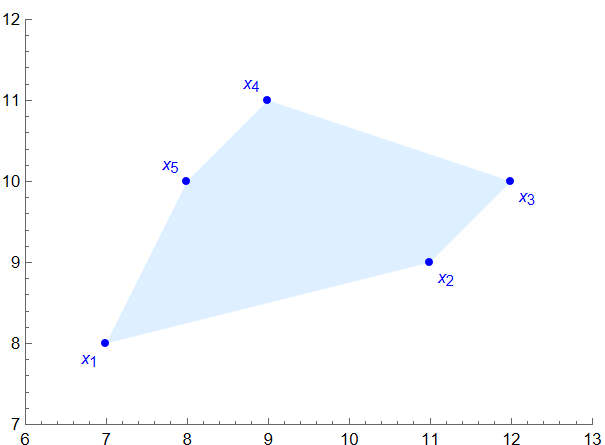
\includegraphics[scale=0.7]{P}
\end{figure}

Нека първо разгледаме правата минаваща през $x_1$ и $x_2$. Наклонът е $\frac{9-8}{11-7}=\frac{1}{4}$ и съответно свободния член е $\frac{25}{4}$. Съответно получаваме уравнение на права $y = \frac{1}{4}x+\frac{25}{4}$, което можем да преобразуваме като $x - 4y = -25.$. Трябва да вземем полуравнината, в която се намират останалите точки. Нека използваме $x_3$. $12-40=-28<-25$, съответно финалното неравенство, което ще включим към израза е $x-4y\leq-25$. Аналогично правим и за останалите прави и получаваме:
\[P=
\left\{
\begin{array}{l}
	x-4y\leq-25\\
	x-y\leq2\\
	x+3y\leq42\\
	x-y\geq-2\\
	2x-y\geq6
\end{array}
\right.
\]
Можем да направим проверка с точка $(10,10)$ и виждаме, че изпълнява всички неравенства.\\

\textbf{Задача 2.}

Получено е следното решение от Excel:

\begin{figure}[h]
	\centering
	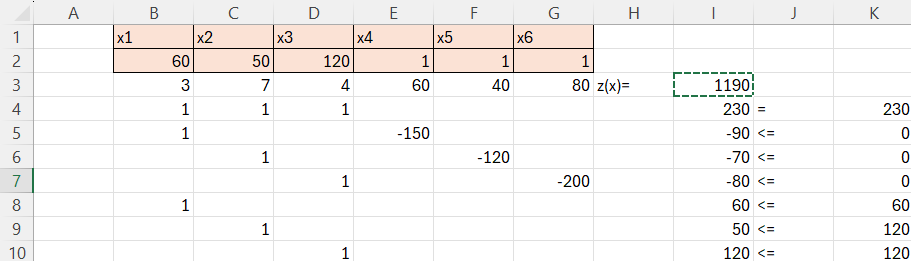
\includegraphics[scale=0.7]{exc}
\end{figure}

\indent \textbf{a)} Оптималната стойност на целевата функция е 1190 и оптималното решение е $\overline{x}=(60,50,120,1,1,1)$\\
\indent \textbf{б)} Настройките са следните:

\begin{figure}[h]
	\centering
	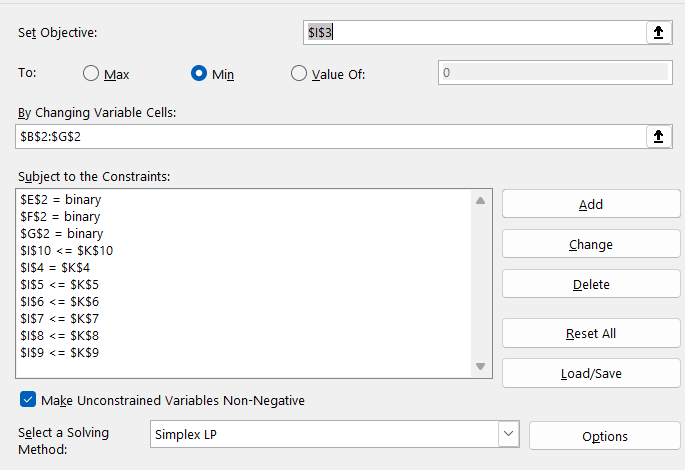
\includegraphics[scale=0.9]{set}
\end{figure}

\indent \textbf{в)}

\begin{figure}[h]
	\centering
	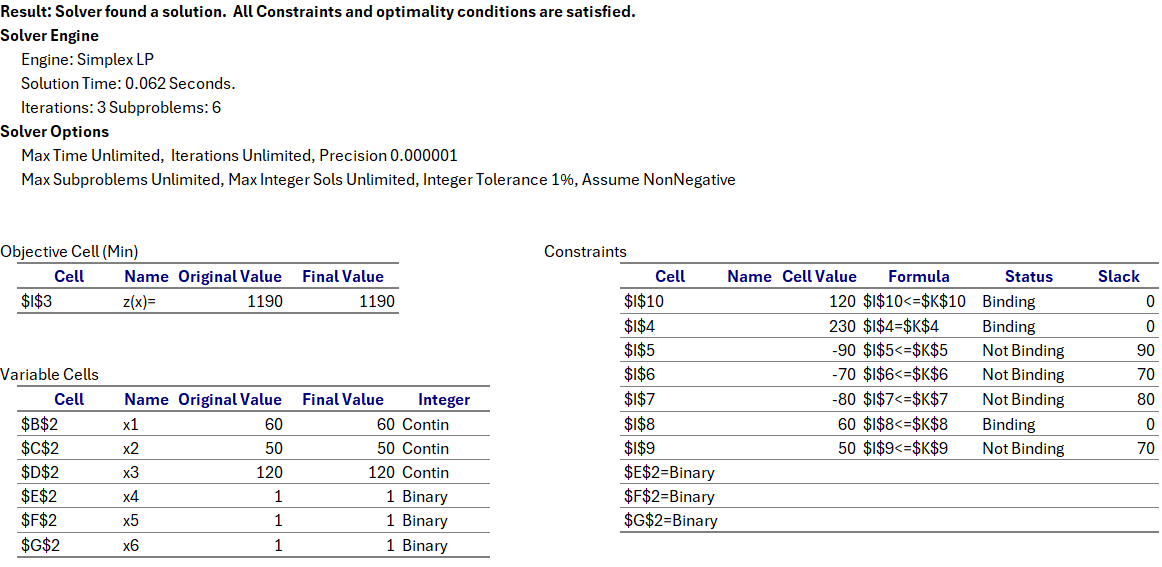
\includegraphics[scale=0.7]{rep}
\end{figure}

\indent \textbf{г)} Да, както е показано в горната справка имаме 4 пасивни ограничения, които са всички без $x_3\leq120$, $x_1\leq60$ и равенството.





\end{document}